% What kind of text document should we build
\documentclass[a4,10pt]{article}


% Include packages we need for different features (the less, the better)	
\usepackage{cleveref}

% Math
\usepackage{amsmath}

% Algorithms
\usepackage{algorithm}
\usepackage{algpseudocode}
\usepackage{comment}
\usepackage{url}
\usepackage{float}

% Tikz
\RequirePackage{tikz}
\usetikzlibrary{arrows,shapes,calc,through,intersections,decorations.markings,positioning}

\tikzstyle{every picture}+=[remember picture]

\RequirePackage{pgfplots}


% Set TITLE, AUTHOR and DATE
\title{A Project Report on Applied Geometry and Special Effects}
\author{James Pandey}
\date{\today}

\begin{document}

% Create the main title section
\maketitle
\begin{center}
  \url{https://github.com/pandeyjames/AppGeoMod}
 \end{center}
\begin{abstract}
This document is a Project Report on the assigned task for STE6247- Applied Geometry and Special Effects.

This report contains the details of how the given assignment was finalized with creating the support class for the curves, splines and surfaces to demonstrate how they exactly can be build in Geometrical Modeling and to know the possibility of their mathematical model to be implemented.
The task is done using hardcoded mathematical operations rather than advance option that is already available in GMlib. The functional attributes of curves and B-Spline Curves, and BSpline Surfaces created and demonstrated, including some basic algorithms and methods.

The application depends on GMlib, Geometric Modeling Library v 0.6.9, and the Qt development suite.
The basic setup template for the task was taken from gmlibqmldemo application and further on the task assigned to implement our own curves and surfaces.
\end{abstract}


%%%%%%%%%%%%%%%%%%%%%%%%%%%%%%%%%%%%%%
%%  The main content of the report  %%
%%%%%%%%%%%%%%%%%%%%%%%%%%%%%%%%%%%%%%


%	  \section{Introduction}
%            The theoritical background of programming in C++ ~\cite{wesley:2013} is achieved during earlier studies.
%            Here it is a practical bases of the theories which were studied in the past now has a direct implementation using guide and nomenclature of Qt platform~\cite{guide:2016}
%	    The C++ programming language comes with a standard library, the \emph{Standard Template Library} (STL), which consists of containers, methods, algorithms and more.
%	
%	    Qt (usually pronounced as "cute",) is used mainly for developing application software with graphical user interfaces (GUIs);
%	    however, programs without a GUI can be developed, such as command-line tools and consoles for servers.
%	    Qt is a cross-platform application framework that is widely used
%            for developing application software that can be run on various software and hardware platforms with little or no
%            change in the underlying code-base, while still being a native application with the capabilities and speed thereof. Using Qt framework with the Gmlib via GLEW 2.0
%            an openGl framework a different approach to Graphic Project is carried out.
%	  
%            %The demonstration of the output of the program, (see \cref{fig:first_demo}).
%	    
%            \begin{figure}[ht]
%	      \centering
%              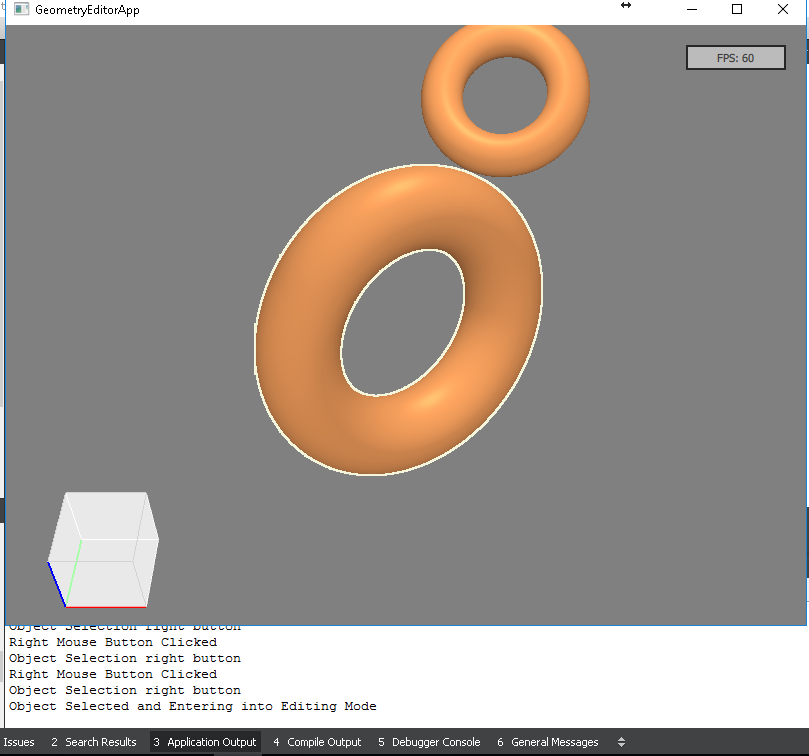
\includegraphics[width=0.8\textwidth]{gfx/first_demo.png}
%	      \caption{Demonstration of the Application selection of the object}
%	      \label{fig:first_demo}
%	    \end{figure}




\section{Introduction}
The project was working created on C++ ~\cite{wesley:2013} and Qt ~\cite{guide:2016} platform with modeling library GMlib.
According to the assignment we have 6 set of tasks to work on, first with the model curve we just take an example for the model curve and try to draw our model curve in using the equations to draw our model curve. I used a 3D Model curve~\cite{ModelCurve} from the website of the University of Rhode Island, Department of Mathematics have developed. After implementing the 1st task move on with the Bspline curve using the Bfunction. The model curve was then modified with Bfunction and then it was created as the Bspline curve generating the knot vectors of the curve.
The same curve of two different example was created to implement the blending of two curves in task 3. In this the part of the 1st curve was blended with the part of the 2nd curve.
For task 4 we have our own GERBS curve which take a model curve and number of the parts for the curve and then the curve is plotted in that amount of number of the parts. They can be individually modified and animated using some basic animation features I have just created a simple animation which rotates the curves parts in x,y and z direction.
The 5th task was to work on with the surfaces as like curves where we have parts of the surfaces that can be modified individually same as curves we have sub-surfaces of the whole surface in plotted and with the control points of the parts of the surface it can be directed and modified.
Task 6 is to work on with the animation of the project that it look good to view on.
All the task completed with provided references and instruction from the Blendbook~\cite{BlendBook:2012}.

\section{Task 1}
Just with the quick start a model curve was taken, then a example file of PCircle from GMlib was grabbed and turned to plot our model curve with the equation taken from the example curve\cref{fig:model} from ~\cite{ModelCurve}.
As it's an individual project the model curve we have taken is all different, needed should focus each and every aspect of the project. A figure below shows the parameters and the attributes of the model curve  that I have chosen but, I have set the value of $t=2\Pi$ to only $\Pi$.
\begin{figure}[h!]
\centering
\includegraphics[width=0.65\textwidth]{gfx/ModelCurve.PNG}
\caption{Attributes of the model curve}
\label{fig:modelcurve}
\end{figure}
\begin{figure}[H]
\centering
\includegraphics[width=0.65\textwidth]{gfx/Model.PNG}
\caption{Curve plotted in the project as open curve from $t=0 $ to $t=\pi $}
\label{fig:model}
\end{figure}

\section{Task 2}
In task 2 we focused to make a B-spline curve from our model curve basically B-spline curve is a spline function which has knot vectors at equal distance and that it can be used for
curve-fitting and numerical-differentiation of data from experiments.
The model curve from task 1 is taken and implemented for the model version of a 2nd degree B-spline curve
the class usage, PCurve class from GMlib as the base class. The evaluator only need to compute the value. And two constructor according to the assigned task is implemented.


%MyB-spline( const DVector<Vector<float,3>>& c);             // use c as control points - and generate a knotvector
%MyB-spline( const DVector<Vector<float,3>>& p, int n);     // use least square to make n control points - and generate a knotvector

\begin{figure}[h!]
	\centering
	\includegraphics[width=0.45\textwidth]{gfx/bspline.png}
	\includegraphics[width=0.45\textwidth]{gfx/bsplinemodified.png}
	\caption{Bspline curves, with selectors manipulation}
	\label{fig:spline}
\end{figure}
\section{Task 3}
Blending of two curves, the first part of a curve is blended with the part of the second curve, we have used the B-function which slightly changes the original curve to blend with another curve
Bfunction only changes the value of the curves but it is approximately same as the first curve. Here the 1st and second curve is inserted as parameter and how much part want to be blended.

Implementation of the curve resulting from blending two curves with a B-function over a given part of the two curves for e.g. 0.3 of 1st curve and 0.7 of 2nd curve.

\begin{figure}[h!]
	\centering
	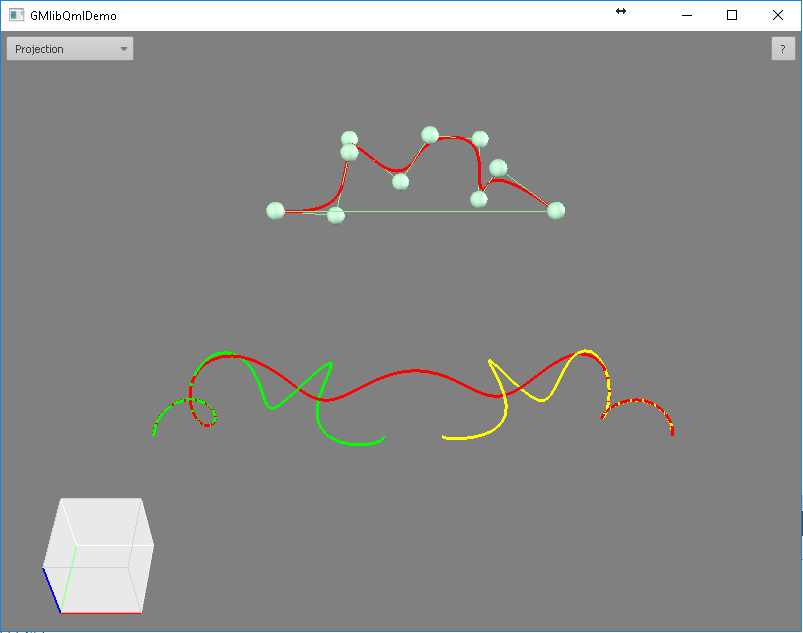
\includegraphics[width=0.70\textwidth]{gfx/blendingcurves.png}
	\caption{Blending of the two curves}
	\label{fig:blendingcurve}
\end{figure}
\section{Task 4}
In task 4 there is to be implmented own version of GERBS curve of the blending spline type where we this gerbs parts and animate them individually. For the subcurves of the model curve
GMlib's PSubCurve class was used to make the local curves. And the same model curve from the 1st part was modeled as GERBS.

\begin{figure}[H]
	\centering
	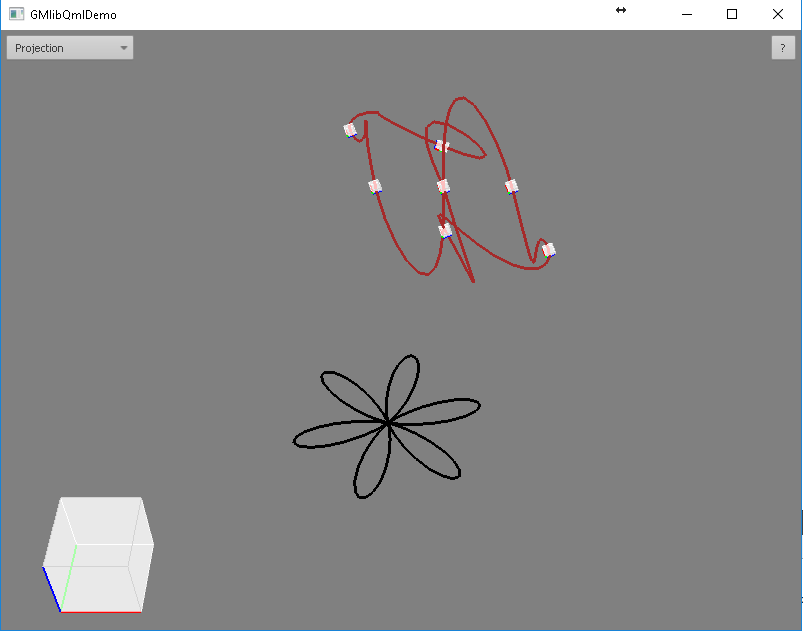
\includegraphics[width=0.45\textwidth]{gfx/gerbcurve1.png}
	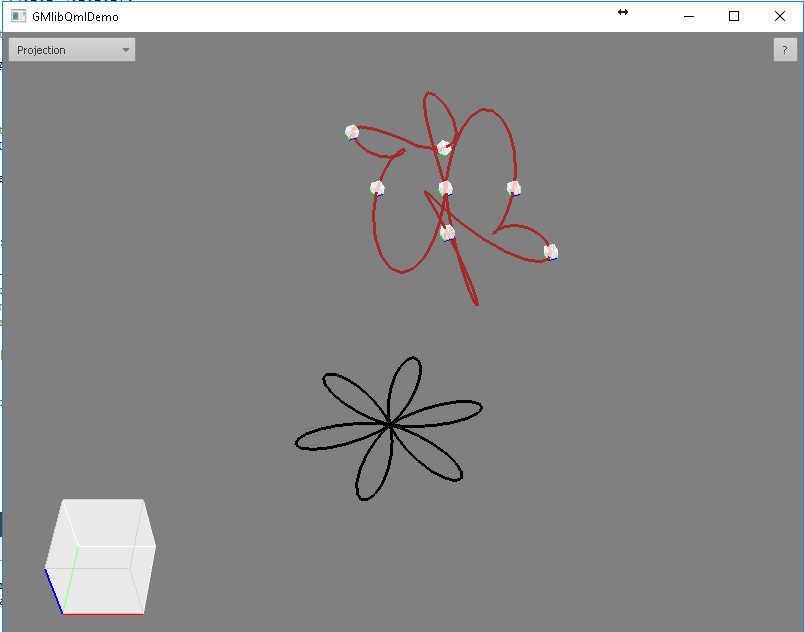
\includegraphics[width=0.45\textwidth]{gfx/gerbcurve2.png}
	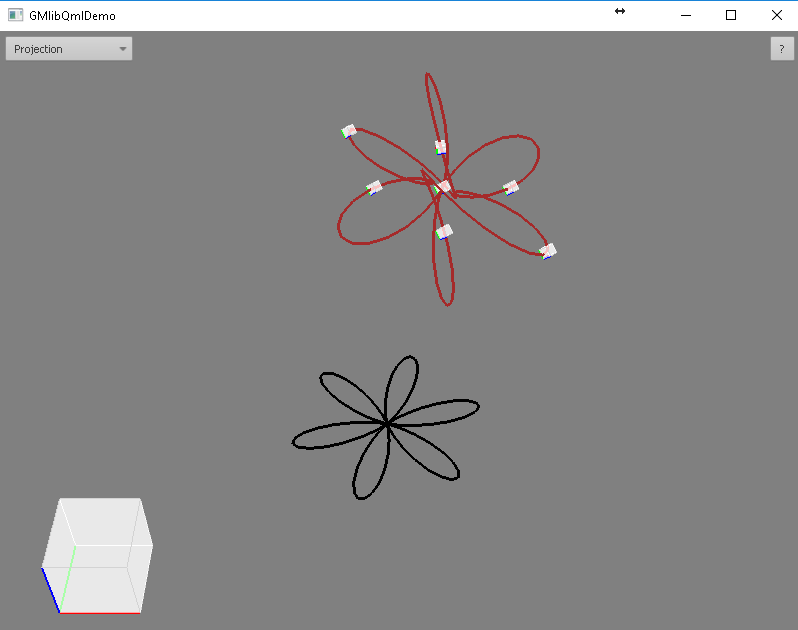
\includegraphics[width=0.45\textwidth]{gfx/gerbcurve3.png}
	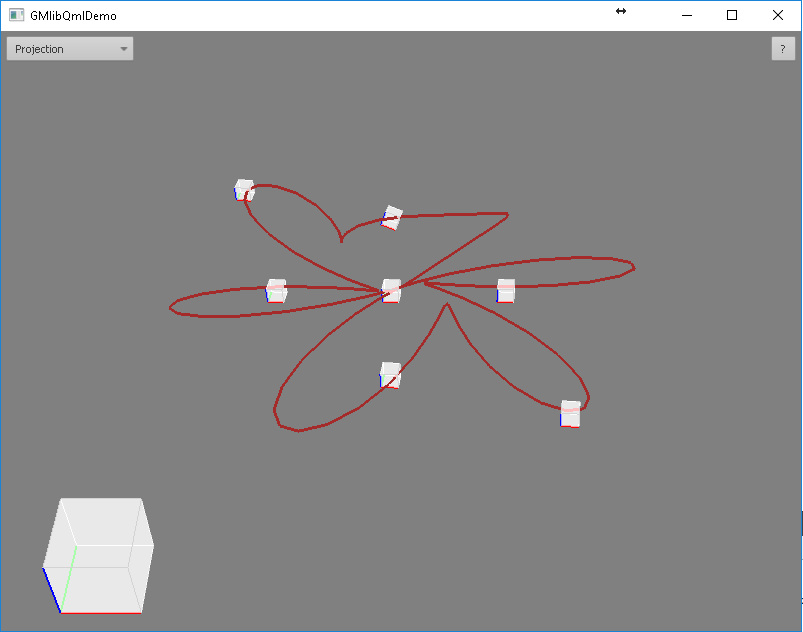
\includegraphics[width=0.45\textwidth]{gfx/gerbcurve4.png}
	\caption{GERBS curve in animation snaps}
	\label{fig:gcurve}
\end{figure}

\section{Task 5}
As of in task 4 here we used surfaces to build the GERBS surface of blending spline type. But we have used SimpleSubSurf class externally provided to make it the more simpler version than
the existing one in GMlib. We just calculated 1st derivative of the B-function for this. And it was done for both open and closed surfaces. A plane is an example of open surface while Cylinder is
closed in one direction and open in other direction. Simple transformation of the surfaces is possible, where the control points like functions as replacers, small cube boxed on the surface is enabled when when we set the flag setCollapsed() to true for the sub-surfaces.
We can select that receptor points and edit our local surfaces and they behave according to the changes.
We can look at the figures of plane \cref{fig:plane} and sphere \cref{fig:sphere} as open and closed surfaces.

\begin{figure}[H]
	\centering
	\includegraphics[width=0.45\textwidth]{gfx/Plane1.png}
	\includegraphics[width=0.45\textwidth]{gfx/Plane2.png}
	\caption{Plane as open GERBS surface, with manipulation}
	\label{fig:plane}
\end{figure}
\begin{figure}[H]
	\centering
	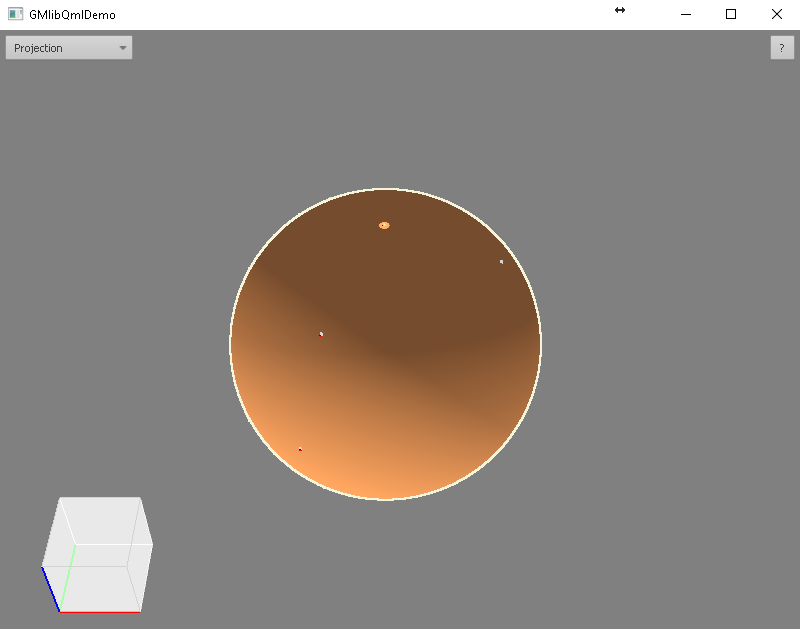
\includegraphics[width=0.45\textwidth]{gfx/sph1.png}
	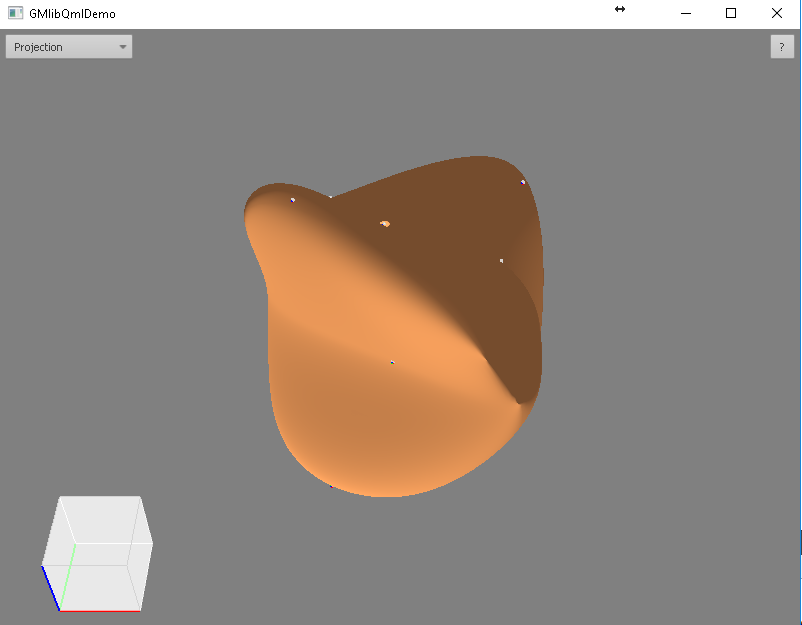
\includegraphics[width=0.45\textwidth]{gfx/sph2.png}
	\caption{Sphere as closed in 1 direction surface and manipulation}
	\label{fig:sphere}
\end{figure}

\section{Task 6}
For the animation portion we can just rotate the parts of the curves and surfaces to give a feel like nice random movements. The part of the local curve and surface they have their own local axis and they can be manipulated within their axis, it just gives us the option
to create animated object of the model. If there were no sub-surfaces or sub-curves then to animate them is not possible, if we apply rotation or translation to the model curve then it will rotate or translate around its own axis, and within it local boundary their is its sub-curves and surfaces
which also rotates with it. But if we apply rotation and translation only to the sub surfaces then the whole model is fixed in the frame and the childs surfaces or the curves will rotate or translate.



%\begin{figure}[]
%\centering
%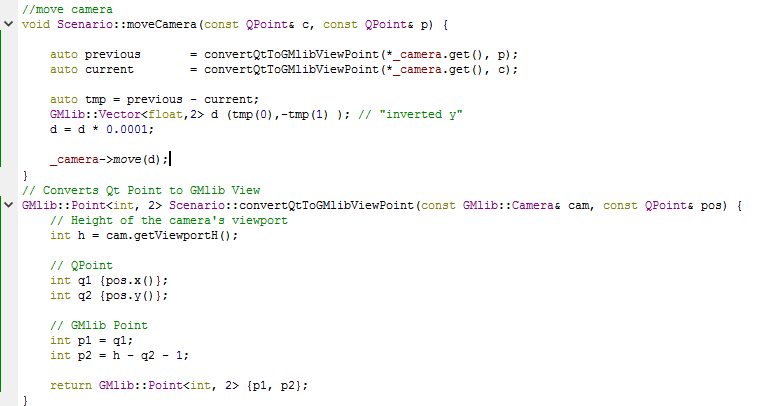
\includegraphics[width=1\textwidth]{gfx/movecamera.png}
%\caption{Codes to handle camera movement}
%\label{fig:movecamera}
%\end{figure}
%\begin{figure}[]
%\centering
%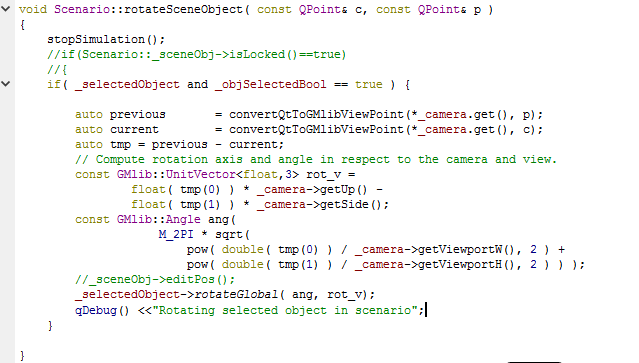
\includegraphics[width=1\textwidth]{gfx/rotateobject.png}
%\caption{Codes to rotate scene object}
%\label{fig:rotateobject}
%\end{figure}
%\begin{figure}[]
%\centering
%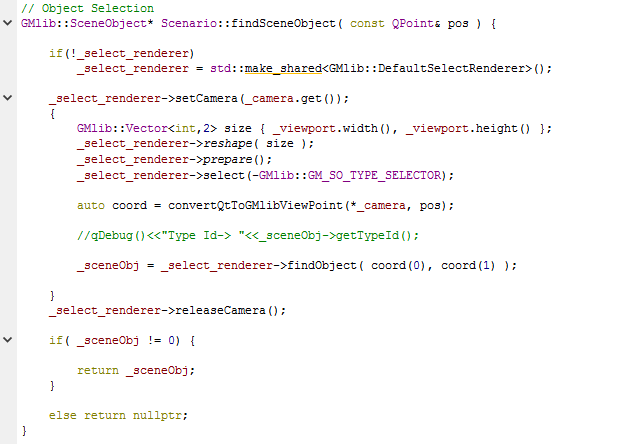
\includegraphics[width=1\textwidth]{gfx/select.png}
%\caption{Codes to select object on the screen}
%\label{fig:rotateobject}
%\end{figure}
%\begin{figure}[]
%\centering
%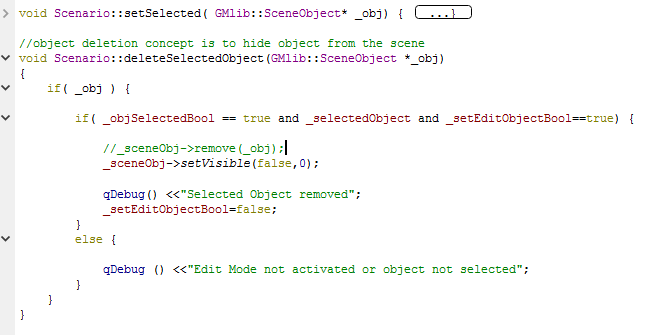
\includegraphics[width=1\textwidth]{gfx/deleteobject.png}
%\caption{Codes to delete object on the screen}
%\label{fig:rotateobject}
%\end{figure}
\pagebreak




\section{Conclusion}
Each and every task are completed from task 1 to 6, works for both open and closed curves and open and closed surfaces with 1st derivative to replot surfaces.
  Future enhancements may include array of object insertion to the scene manipulation with ease and creating a live object like a car, snowman, with the surfaces added and various editing functions like scale, resize, delete, insert, with multiple type of object.
  A features of saving and loading of the curves and surfaces that are in the seen to the computer and then retrieving them back to scene will be so exciting for add-up.

% Include the bibliography
\bibliographystyle{plain}
\bibliography{bibliography}

\end{document}
